\documentclass[12pt, letterpaper]{article}

%-------Packages---------
\usepackage{amssymb,amsfonts}
\usepackage{amsthm}
\usepackage{graphicx}
\usepackage[all,arc]{xy}
\usepackage{enumerate}
\usepackage{bbm}
\usepackage{dsfont}
\usepackage{mathrsfs}
\usepackage{tikz-cd}
\usepackage{setspace}
\usepackage{import}
\usepackage[utf8]{inputenc}
\usepackage{hyperref}
\usepackage{tikz}
\usepackage{float}
\usepackage[dvipsnames]{xcolor}
\usepackage[nocheck]{fancyhdr}
\usepackage[nointegrals]{wasysym}

\usepackage[left=1in,top=1in,right=1in,bottom=1in]{geometry}

\usepackage{mathtools}
\usepackage{setspace}
\usepackage{cleveref}
\usepackage{multicol}
\usepackage{mathpazo}
\usepackage{xparse}

\usepackage[all]{xypic}
\usepackage{xcolor, ifthen, tcolorbox}
\tcbuselibrary{theorems,skins,breakable}
% Theorem System
% The following environments are provided:
%   New Problem:        \begin{problem} ...
%   New Question Header:   \qh (then followed by subproblems)
%   Subproblem:     \begin{subproblem} ...
%   Problem Proof:  \begin{problemproof} ...
%   Proof:          \\begin{pf}{color} ...
%   Remark:         \rmk (sentence), \rmkb (block)

% Define custom colors
\definecolor{thmscol}{HTML}{F4565B} %For Problems
\definecolor{lemscol}{HTML}{FE844C} %For Lemmes
\definecolor{prpscol}{HTML}{00A7EF} %For proposition
\definecolor{corscol}{HTML}{23DAFF} %For corrolaries
\definecolor{rmkscol}{HTML}{6DEEC5} %For remarks
\definecolor{defscol}{HTML}{18C991} %For definitions
\definecolor{exmscol}{HTML}{7DB800} %For examples
\definecolor{clmscol}{HTML}{165c58} %For claims

%Change between dark(black)/light(white) mode
\newcommand{\colormode}{white}
\ifthenelse{\equal{\colormode}{white}}
      {\newcommand{\TextColor}{black}}
      {\newcommand{\TextColor}{white}}
\newcommand{\pbcolormain}{thmscol!80!\colormode}
\newcommand{\pbcolorsecond}{thmscol!38!\colormode}


% ============================
% Problem Counter
% ============================
\newcounter{subproblemcounter}
\newcounter{problemcounter}

\newcommand{\q}{
    \setcounter{subproblemcounter}{0}%
    \stepcounter{problemcounter} % Increment problem counter
    \color{\TextColor}Problem \arabic{problemcounter}: % Display the problem counter
}

\newcommand{\stepsub}{
    \stepcounter{subproblemcounter}%
    \color{\TextColor}(\alph{subproblemcounter})
}
% ============================
% Problem
% ============================
\newtcolorbox{pb}[1]{
  enhanced,
  frame hidden,
  titlerule=0mm,
  toptitle=1mm,
  bottomtitle=1mm,
  fonttitle=\bfseries\large,
  coltitle=black,
  colbacktitle=\pbcolormain,
  colback=\pbcolorsecond,
  title={\q #1},
  coltext=\TextColor
}

\newtcolorbox{spb}[1]{
  enhanced,
  frame hidden,
  titlerule=0mm,
  toptitle=1mm,
  bottomtitle=1mm,
  fonttitle=\bfseries\large,
  coltitle=black,
  colbacktitle=\pbcolormain,
  colback=\pbcolorsecond,
  title={\stepsub #1},
  coltext=\TextColor,
  attach boxed title to top left={xshift=3mm,yshift=-2mm},
  boxed title style={
    colback=\pbcolormain,
    colframe=\pbcolormain,
  }
}

\newtcolorbox{pbh}[1]{
    enhanced,
    frame hidden,
    titlerule=0mm,
    toptitle=1mm,
    bottomtitle=1mm,
    fonttitle=\bfseries\large,
    coltitle=black,
    colbacktitle=\pbcolormain,
    colback=\pbcolorsecond,
    title={\q #1},
    boxrule=0pt,
    interior hidden,
    attach boxed title to top left={xshift=3mm,yshift=-2mm},
    boxed title style={
        colback=\pbcolormain,
        colframe=\pbcolormain,
    }
}

\newenvironment{problem}[1]{%
  \newpage
  \begin{pb}{#1}
    }{
  \end{pb}
}

\newenvironment{subproblem}[1]{%
  \begin{spb}{#1}
    }{
  \end{spb}
}

\newenvironment{problemproof}{%
    \begin{pf}{\pbcolormain}
        }{
    \end{pf}
}

\newcommand{\qh}[1][]{
    \newpage
    \begin{pbh}{#1}\end{pbh} % Display the problem counter
}

% ============================
% Claim
% ============================

\newtcbtheorem[number within=problemcounter]{claim}{Claim}
{
    enhanced,
    frame hidden,
    titlerule=0mm,
    toptitle=1mm,
    bottomtitle=1mm,
    fonttitle=\bfseries\large,
    coltitle=black,
    colbacktitle=clmscol!50!\colormode,
    colback=clmscol!20!\colormode,
}{clm}

\NewDocumentCommand{\clm}{m+m}{
    \begin{claim*}{#1}{}
        #2
    \end{claim*}
}

\newenvironment{clmpf}{
	{\noindent{\it \textbf{Proof.}}
	\setlength{\parindent}{0pt}
	}
	\tcolorbox[blanker,breakable,left=5mm,parbox=false,
    before upper={\parindent15pt},
    after skip=10pt,
	borderline west={1mm}{0pt}{clmscol!50!\colormode}]
}{
    \textcolor{clmscol!50!\colormode}{\hbox{}\nobreak\hfill$\blacksquare$}
    \endtcolorbox
}

\NewDocumentCommand{\clmp}{m+m+m}{
    \begin{claim*}{#1}{}
        #2
    \end{claim*}

    \begin{clmpf}
        #3
    \end{clmpf}
}


% ============================
% Proof
% ============================

\newenvironment{pf}[1]{%
  \def\pfcolor{#1}% Store the color in a macro
  \noindent{\it \textbf{Proof.}}%
  \tcolorbox[blanker,breakable,left=5mm,parbox=false,%
    before upper={\parindent15pt},%
    after skip=10pt,%
    borderline west={1mm}{0pt}{\pfcolor},%
    coltext=\TextColor
  ]%
  \setlength{\parindent}{0pt}%
}{%
  \textcolor{\pfcolor}{\hbox{}\nobreak\hfill$\blacksquare$}%
  \endtcolorbox%
}

\newtcolorbox{solution}{
  blanker,
  breakable,
  left=5mm,
  parbox=false,%
  before upper={\parindent15pt},%
  after skip=10pt,%
  borderline west={1mm}{0pt}{\pbcolormain},%
  coltext=\TextColor
}


% ============================
% Remark
% ============================


\NewDocumentCommand{\rmk}{+m}{
    {\it \color{rmkscol!100!white}#1}
}

\newenvironment{remark}{
    \par
    \vspace{5pt}
    \begin{minipage}{\textwidth}
        {\par\noindent{\textbf{Remark.}}}
        \tcolorbox[blanker,breakable,left=5mm,
        before skip=10pt,after skip=10pt,
        borderline west={1mm}{0pt}{rmkscol!80!\colormode},
        coltext=\TextColor
        ]
}{
        \endtcolorbox
    \end{minipage}
    \vspace{5pt}
}

\NewDocumentCommand{\rmkb}{+m}{
    \begin{remark}
        #1
    \end{remark}
}


% Define a new command for problems
\renewcommand{\headrule}{\color{\TextColor}\hrulefill}
\newcommand{\C}{\mathbb{C}}
\newcommand{\R}{\mathbb{R}}
\newcommand{\Q}{\mathbb{Q}}
\newcommand{\Z}{\mathbb{Z}}
\newcommand{\N}{\mathbb{N}}
\renewcommand{\P}{\mathbb{P}}
\newcommand{\F}{\mathbb{F}}
\newcommand{\contr}{\Rightarrow \Leftarrow}
\newcommand{\s}{\(\,\)}
\renewcommand{\t}[1]{\text{#1}}
\newcommand{\ang}[1]{\left\langle #1 \right\rangle}
\newcommand{\coker}{\mathrm{coker}}

% Meta data
\setstretch{1.2}

\begin{document}
\color{\TextColor}
\pagecolor{\colormode}

\renewcommand{\pbcolormain}{clmscol!60!white}
\renewcommand{\pbcolorsecond}{clmscol!30!white}
\renewcommand{\stepsub}{
    \stepcounter{subproblemcounter}%
    \color{\TextColor}\arabic{subproblemcounter}.
}

\setlength{\parindent}{0pt}
\pagestyle{fancy}
\fancyhf{}
\fancyhead[LOE]{\color{\TextColor}\slshape{\textbf{Vincent Ferrara}}}
\fancyhead[ROE]{\color{\TextColor}\thepage}


\qh[Floating point--mind the gap]
\begin{subproblem}{}
    In a 32-bit IEEE floating point number, what is the smallest number greater than 10 that can be exactly represented?  What is the gap between that number and 10?  Briefly justify your answers.
\end{subproblem}
The decimal number 10 is represented in binary as:

\[
10_{10} = 1010_2
\]

We express this in the form:

\[
10_{10} = 1.010_2 \times 10^3
\]

To find the smallest number greater than 10, we take the maximum number of trailing zeros and place a single 1 at the very end. This ensures it is the next representable number larger than 10.

Thus, in IEEE standard, this number is represented as:

\[
0 \quad 1000 \quad 0010 \quad 010 \quad 0000 \quad 0000 \quad 0000 \quad 0000 \quad 0001
\]

This ensures that the number remains as close to 10 as possible while being strictly greater than it. This is equal to $1.01000000000000000000001_2 \times 10^3$. The gap between them is $1010_2-1010.00\cdots1_2=2^{-20}$

\begin{subproblem}{}
    Assuming we are always rounding to the nearest value we can exactly represent (rounding down in the case of ties), what is the largest value we can add to 10 and get a result that is still 10?
\end{subproblem}

For the last part, the largest value that can be added to 10 and still have it round to 10 is \(2^{-21}\). Near 10 in the 32-bit IEEE representation, the gap between consecutive representable numbers is \(2^{-20}\). When rounding to the nearest value (with ties rounding down), any value less than half of that gap—namely, \(2^{-21}\)—won't push the total over the midpoint between 10 and the next representable number, which is \(10 + 2^{-20}\). Thus, even when you add \(2^{-21}\) to 10, the sum is still closer to 10 than to \(10 + 2^{-20}\), ensuring that it rounds back to 10.

\begin{subproblem}{}
    Redo part 1) but for -17.125 rather than 10?.
\end{subproblem}
The decimal number 17.5 is represented in binary as:

\[
17.5_{10} = 10001.001_2
\]

We express this in the form:

\[
17.5_{10} = 1.0001001_2 \times 10^4
\]
Doing the same thing as part 1 we can add the max amount of zeros and place a 1 and the end.
Thus, we get:
\[1 \quad 1000 \quad 0011 \quad 000 \quad 1001 \quad 0000 \quad 0000 \quad 0000 \quad 0001\]
This is equal to $1.00010010000000000000001_2 \times 10^4$. Thus, the gap is $2^{-19}$

\begin{subproblem}{}
    Briefly explain how the gap between floating point numbers might cause a programmer
    difficulties. In particular, consider a for loop where small values are being added to a larger number many thousands of times.
\end{subproblem}
Floating-point numbers have non-uniform spacing; as numbers grow larger, the gap between them increases. This means that when a small value is repeatedly added to a much larger number—say, inside a for loop—the addition might not change the larger number at all because the increment is smaller than the gap between representable numbers. For example, if the increment is less than half the gap, it may be effectively “lost” due to rounding, and the running total may remain unchanged for many iterations. This can lead to unexpected behavior and accumulated errors in calculations, posing a significant challenge in numerical computations and simulations.

\begin{problem}{Linking}
    If a global variable is declared in a source file named file1.c, do accesses to it in file1.c need to go
in the relocation table when linking? Why or why not? Briefly explain your answer.
\end{problem}
No, they don't. When file1.c is compiled, the compiler already figures out the exact location of the global variable in that file. 
This means that any reference to the variable within file1.c already knows where to go, so there's no need for the linker to adjust these addresses later using the relocation table.

\begin{problem}{Multiplication-by-wire}
    Say you have a 4-bit unsigned number $X[3:0]$ (so $X_3$ is the most significant bit, $X_2$ is the next most significant, etc.). 
    Using only standard gates (AND, OR, NOT), and constant 0s and 1s, multiply $X[3:0]$ by 8.5 and output it as an 8-bit unsigned number $Y[7:0]$. Use as few gates as possible, even if it means you use no gates. You may assume that $X$ is divisible by 2.
\end{problem}
\begin{center}
    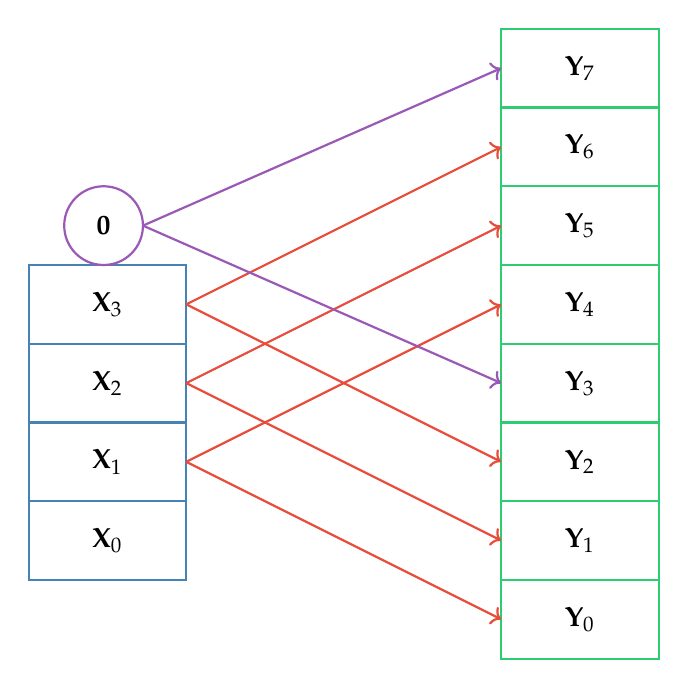
\begin{tikzpicture}
        % Define colors
        \definecolor{inputcolor}{RGB}{70, 130, 180}  % Steel Blue
        \definecolor{outputcolor}{RGB}{46, 204, 113} % Emerald Green
        \definecolor{arrowcolor}{RGB}{231, 76, 60}   % Red
        \definecolor{zerocolor}{RGB}{155, 89, 182}   % Purple

        % Draw input box for X
        \draw[inputcolor, thick] (0,4) rectangle (2,5) node[pos=.5, black] {\textbf{X$_3$}};
        \draw[inputcolor, thick] (0,3) rectangle (2,4) node[pos=.5, black] {\textbf{X$_2$}};
        \draw[inputcolor, thick] (0,2) rectangle (2,3) node[pos=.5, black] {\textbf{X$_1$}};
        \draw[inputcolor, thick] (0,1) rectangle (2,2) node[pos=.5, black] {\textbf{X$_0$}};

        % Draw zero circle
        \node[draw, circle, minimum size=1cm, thick, zerocolor, text=black] at (0.95,5.5) {\textbf{0}};
    
        % Draw output box for Y
        \draw[outputcolor, thick] (6,7) rectangle (8,8) node[pos=.5, black] {\textbf{Y$_7$}};
        \draw[outputcolor, thick] (6,6) rectangle (8,7) node[pos=.5, black] {\textbf{Y$_6$}};
        \draw[outputcolor, thick] (6,5) rectangle (8,6) node[pos=.5, black] {\textbf{Y$_5$}};
        \draw[outputcolor, thick] (6,4) rectangle (8,5) node[pos=.5, black] {\textbf{Y$_4$}};
        \draw[outputcolor, thick] (6,3) rectangle (8,4) node[pos=.5, black] {\textbf{Y$_3$}};
        \draw[outputcolor, thick] (6,2) rectangle (8,3) node[pos=.5, black] {\textbf{Y$_2$}};
        \draw[outputcolor, thick] (6,1) rectangle (8,2) node[pos=.5, black] {\textbf{Y$_1$}};
        \draw[outputcolor, thick] (6,0) rectangle (8,1) node[pos=.5, black] {\textbf{Y$_0$}};
    
        % Draw arrows for the mappings
        \draw[->, thick, arrowcolor] (2,4.5) -- (6,6.5); % X3 to Y6
        \draw[->, thick, arrowcolor] (2,4.5) -- (6,2.5); % X3 to Y2

        \draw[->, thick, arrowcolor] (2,3.5) -- (6,5.5); % X2 to Y5
        \draw[->, thick, arrowcolor] (2,3.5) -- (6,1.5); % X2 to Y1

        \draw[->, thick, arrowcolor] (2,2.5) -- (6,4.5); % X1 to Y4
        \draw[->, thick, arrowcolor] (2,2.5) -- (6,0.5); % X1 to Y0

        % Arrows from zero circle
        \draw[->, thick, zerocolor] (1.45,5.5) -- (6,7.5); % Zero to Y7
        \draw[->, thick, zerocolor] (1.45,5.5) -- (6,3.5); % Zero to Y3

    \end{tikzpicture}
\end{center}
This approach works by breaking the multiplication by 8.5 into two separate steps: first multiplying by 8 and then by 0.5, before combining the results. 
Multiplying by 8 in binary is equivalent to shifting all bits left by three positions, which moves \( X_3 \) to \( Y_6 \), \( X_2 \) to \( Y_5 \), and \( X_1 \) to \( Y_4 \), while \( X_0 \), which is always 0 because \( X \) is given to be divisible by 2, shifts into \( Y_3 \), which is also set to 0. Similarly, multiplying by 0.5 is equivalent to shifting all bits right by one position, moving \( X_3 \) to \( Y_2 \), \( X_2 \) to \( Y_1 \), and \( X_1 \) to \( Y_0 \), with \( X_0 \) being dropped entirely. 
Since the results from these two shifts do not overlap in \( Y[7:0] \), we can simply place the shifted values in their respective positions without needing to add or modify any bits. 
The remaining positions in \( Y \) that are not assigned by either shift—specifically \( Y_7 \) and \( Y_3 \)—are set to 0. 
Because this transformation is achieved entirely through bit shifting and direct wiring, there is no need for additional logic gates, making this an efficient and minimal implementation. 
The fact that \( X_0 \) is always 0 further simplifies the process, ensuring that no extra handling is needed for that bit during shifting operations.

\begin{problem}{Latches and flip-flops}
    Complete the timing diagrams for a D latch and D flip-flop given the provided inputs. 
    The flip-flop is positive-edge triggered. For the latch we are using “C” for the “G” input (which is fairly common).
    Assume both the latch and the flip-flop have an initial value of zero
\end{problem}
\begin{center}
    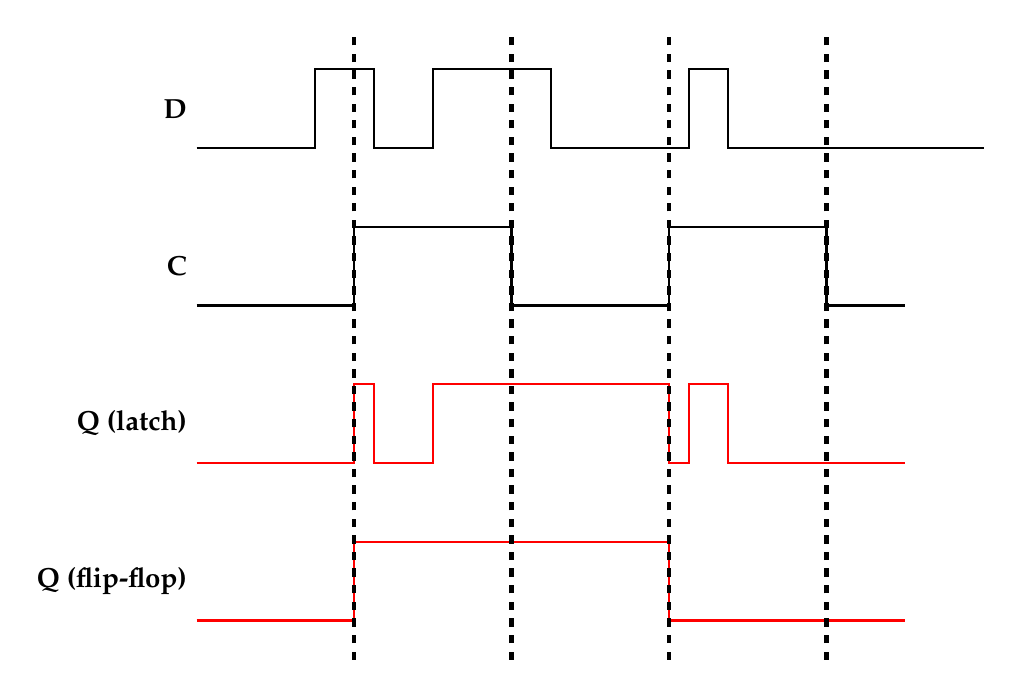
\begin{tikzpicture}
        % D Signal (topmost)
        \draw[thick] (0,8) -- (1.5,8) -- (1.5,9) -- (2.25,9) -- (2.25,8) -- (3,8) -- (3,9) -- (4.5,9) -- (4.5,8) -- (6.25,8) -- (6.25,9) --(6.75,9) -- (6.75,8) -- (10,8);
        \node[left] at (0,8.5) {\textbf{D}};
    
        % Clock (C) Signal (shifted downward for more spacing)
        \draw[thick] (0,6) -- (2,6) -- (2,7) -- (4,7) -- (4,6) -- (6,6) -- (6,7) -- (8,7) -- (8,6) -- (9,6);
        \node[left] at (0,6.5) {\textbf{C}};
    
        % Q (latch) Output (spaced further below)
        \draw[red, thick] (0,4) -- (2,4) -- (2,5) -- (2.25,5) -- (2.25,4) -- (3,4) -- (3,5) -- (6,5) -- (6,4) -- (6.25,4) -- (6.25,5) -- (6.75,5) -- (6.75,4) -- (9,4);
        \node[left] at (0,4.5) {\textbf{Q (latch)}};
    
        % Q (flip-flop) Output (spaced furthest below)
        \draw[red, thick] (0,2) -- (2,2) -- (2,3) -- (6,3) -- (6,2) -- (9,2);
        \node[left] at (0,2.5) {\textbf{Q (flip-flop)}};
    
        % Dashed vertical lines for clock edges (now 4 dashed lines, ultra thick)
        \foreach \x in {2,4,6,8} {
            \draw[dashed, ultra thick] (\x,1.5) -- (\x,9.5);
        }
    
    \end{tikzpicture}
\end{center}

\qh[State machines]
\begin{subproblem}{}
    Consider a state machine implementation with 6 state bits. 
    What is the maximum number of states you can have with such an implementation?
\end{subproblem}
A state machine with 6 state bits can represent a maximum of \(2^6 = 64\) unique states, as each bit can be either 0 or 1, resulting in \(2^6\) possible combinations.

\begin{subproblem}{}
    Say you have a state machine with 5 bits of input, 3 bits of output, and 24 states. How large would your control ROM need to be? Fill in the blanks below.
\end{subproblem}
\begin{center}
    \large 10 bits of address\\
    8 bits data per address\\
    A total of $2^{13}$ bits in the ROM.
\end{center}

\begin{problem}{Incremental Improvement}
    In a moment of clarity, the EECS 370 staff realizes that the LC2K instruction set is rather limited in its capability to take advantage of the AI boom. 
    To improve the situation, the EECS 370 staff decides to implement a new instruction: load from pointer (LFP). The semantics of the LFP instruction are provided below.
\end{problem}
\begin{center}
    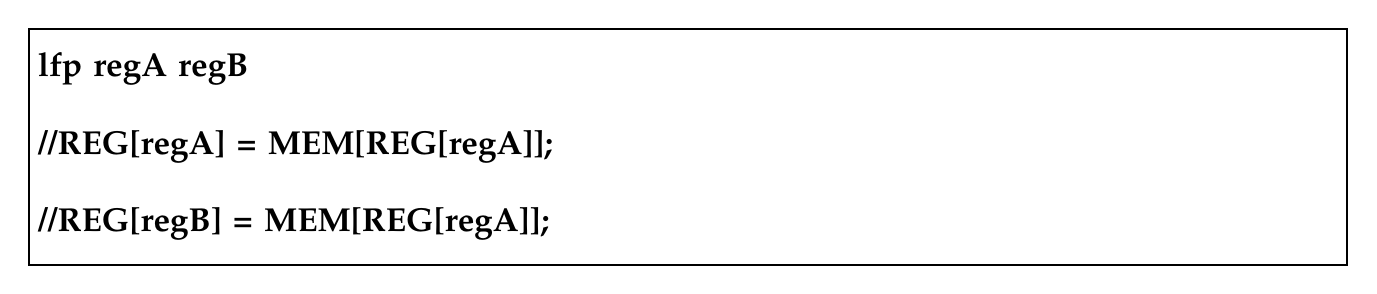
\begin{tikzpicture}
        \node[draw=black, thick, font=\bf\large, align=left, text width=6.5 in, minimum height=3cm] 
        at (0,0) {lfp regA regB \\
        \phantom{text}\\
        //REG[regA] = MEM[REG[regA]];\\
        \phantom{text}\\
        //REG[regB] = MEM[REG[regA]];\\};
    \end{tikzpicture}
\end{center}
\begin{center}
    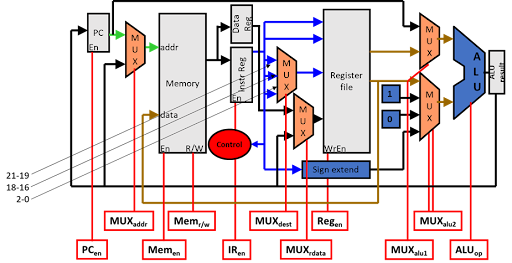
\includegraphics[width=\columnwidth]{pictures/LC2Kdatapath.png}
\end{center}
\begin{table}[H]
    \begin{tabular}{|l|l|l|l|l|l|l|l|l|l|l|l|}
    \hline
    Cycle & \begin{tabular}[c]{@{}l@{}}PC\\ (en)\end{tabular} & \begin{tabular}[c]{@{}l@{}}MUX\\ (addr)\end{tabular} & \begin{tabular}[c]{@{}l@{}}Mem\\ (en)\end{tabular} & \begin{tabular}[c]{@{}l@{}}Mem\\ (r/w)\end{tabular} & \begin{tabular}[c]{@{}l@{}}IR\\ (en)\end{tabular} & \begin{tabular}[c]{@{}l@{}}MUX\\ (dest)\end{tabular} & \begin{tabular}[c]{@{}l@{}}MUX\\ (rdata)\end{tabular} & \begin{tabular}[c]{@{}l@{}}Reg\\ (en)\end{tabular} & \begin{tabular}[c]{@{}l@{}}MUX\\ (alu1)\end{tabular} & \begin{tabular}[c]{@{}l@{}}MUX\\ (alu2)\end{tabular} & \begin{tabular}[c]{@{}l@{}}ALU\\ (op)\end{tabular} \\ \hline
    1     & 0                                                 & 0                                                    & 1                                                  & 0                                                   & 1                                                 & XX                                                   & X                                                     & 0                                                  & 0                                                    & 01                                                   & 0                                                  \\ \hline
    2     & 1                                                 & X                                                    & 0                                                  & X                                                   & 0                                                 & XX                                                   & X                                                     & 0                                                  & X                                                    & XX                                                   & X                                                  \\ \hline
    3     & 0                                                 & X                                                    & 0                                                  & X                                                   & 0                                                 & XX                                                   & X                                                     & 0                                                  & 1                                                    & 10                                                   & 0                                                  \\ \hline
    4     & 0                                                 & 1                                                    & 1                                                  & 0                                                   & 0                                                 & XX                                                   & X                                                     & 0                                                  & X                                                    & XX                                                   & X                                                  \\ \hline
    5     & 0                                                 & X                                                    & 0                                                  & X                                                   & 0                                                 & 00                                                   & 0                                                     & 1                                                  & X                                                    & XX                                                   & X                                                  \\ \hline
    6     & 0                                                 & X                                                    & 0                                                  & X                                                   & 0                                                 & 01                                                   & 0                                                     & 1                                                  & X                                                    & XX                                                   & X                                                  \\ \hline
    \end{tabular}
\end{table}

\qh[SC/MC Datapath Performance]
\begin{subproblem}{}
    What is the clock period for the single-cycle processor if we only had to support add, halt, beq, and lw? 
\end{subproblem}
Since lw is the longest instruction the clock period would be 24ns.

\begin{subproblem}{}
    What is the clock period for the single-cycle processor if we support all LC2K instructions except jalr?
\end{subproblem}
Well again since lw is the longest instruction the clock period would be 24ns.

\begin{subproblem}{}
    If we can decrease the delay for one of the operations by 25\%, which operation should it be for our single-cycle datapath which supports all LC2K instructions except jalr? 
    What is the clock period after improvement?
\end{subproblem}
    So lw is the longest at 24ns and sw is right behind at 23ns. If we decrease read memory we decrease every instruction by 2, and lw by 4ns, thus we get a clock speed of 21ns since sw is now the longest.

\begin{subproblem}{}
    If we can decrease the delay for one of the operations by 25\%, which operation should it be for our multi-cycle datapath which supports all LC2K instructions except jalr? What is the clock period after improvement? 
\end{subproblem}
Since multi-cycle clock speed is based on the longest stage which is when sw writes to memory we can reduce write memory by 25\% and get a new clock speed of 9ns since no other stage was close to 12ns.

\qh[Intro to Pipelining]
\renewcommand{\stepsub}{
    \stepcounter{subproblemcounter}%
    \color{\TextColor}\alph{subproblemcounter}.
}
\begin{subproblem}{}
    Fill in the timing graph below with the pipeline stage that each instruction is in at the start
of each cycle. Recall that the stages are IF, ID, EX, MEM, WB. The first IF has been
filled in for you.
\end{subproblem}
\begin{table}[H]
    \begin{tabular}{|l|l|l|l|l|l|l|l|l|l|}
    \hline
    Instruction \textbackslash Cycle \# & 0  & 1  & 2  & 3   & 4   & 5   & 6   & 7   & 8  \\ \hline
    add 4 7 1                           & IF & ID & EX & MEM & WB  &     &     &     &    \\ \hline
    lw 0 6 1                            &    & IF & ID & EX  & MEM & WB  &     &     &    \\ \hline
    nor 5 3 3                           &    &    & IF & ID  & EX  & MEM & WB  &     &    \\ \hline
    sw 0 2 8                            &    &    &    & IF  & ID  & EX  & MEM & WB  &    \\ \hline
    halt                                &    &    &    &     & IF  & ID  & EX  & MEM & WB \\ \hline
    \end{tabular}
\end{table}
\begin{subproblem}{}
    Fill in the contents of the pipeline registers at the point in time between cycle A and B.
\end{subproblem}
Cycle 0-1:
\begin{table}[H]
    \begin{tabular}{|ll|}
    \hline
    \multicolumn{2}{|l|}{IF/ID}            \\ \hline
    \multicolumn{1}{|l|}{Opcode:}    & add \\ \hline
    \multicolumn{1}{|l|}{PC Plus 1:} & 1   \\ \hline
    \multicolumn{1}{|l|}{}           &     \\ \hline
    \multicolumn{1}{|l|}{}           &     \\ \hline
    \multicolumn{1}{|l|}{}           &     \\ \hline
    \end{tabular}
    \begin{tabular}{|ll|}
    \hline
    \multicolumn{2}{|l|}{ID/EX}             \\ \hline
    \multicolumn{1}{|l|}{Opcode:}    & noop \\ \hline
    \multicolumn{1}{|l|}{PC Plus 1:} & X    \\ \hline
    \multicolumn{1}{|l|}{regA val:}  & X    \\ \hline
    \multicolumn{1}{|l|}{regB val:}  & X    \\ \hline
    \multicolumn{1}{|l|}{offset:}    & X    \\ \hline
    \end{tabular}
    \begin{tabular}{|ll|}
    \hline
    \multicolumn{2}{|l|}{EX/MEM}            \\ \hline
    \multicolumn{1}{|l|}{Opcode:}    & noop \\ \hline
    \multicolumn{1}{|l|}{aluResult:} & X    \\ \hline
    \multicolumn{1}{|l|}{}           &      \\ \hline
    \multicolumn{1}{|l|}{regB val:}  & X    \\ \hline
    \multicolumn{1}{|l|}{}           &      \\ \hline
    \end{tabular}
    \begin{tabular}{|ll|}
    \hline
    \multicolumn{2}{|l|}{MEM/WB}            \\ \hline
    \multicolumn{1}{|l|}{Opcode:}    & noop \\ \hline
    \multicolumn{1}{|l|}{writeDate:} & X    \\ \hline
    \multicolumn{1}{|l|}{}           &      \\ \hline
    \multicolumn{1}{|l|}{}           &      \\ \hline
    \multicolumn{1}{|l|}{}           &      \\ \hline
    \end{tabular}
\end{table}

Cycle 2-3:
\begin{table}[H]
    \begin{tabular}{|ll|}
    \hline
    \multicolumn{2}{|l|}{IF/ID}            \\ \hline
    \multicolumn{1}{|l|}{Opcode:}    & nor \\ \hline
    \multicolumn{1}{|l|}{PC Plus 1:} & 3   \\ \hline
    \multicolumn{1}{|l|}{}           &     \\ \hline
    \multicolumn{1}{|l|}{}           &     \\ \hline
    \multicolumn{1}{|l|}{}           &     \\ \hline
    \end{tabular}
    \begin{tabular}{|ll|}
    \hline
    \multicolumn{2}{|l|}{ID/EX}             \\ \hline
    \multicolumn{1}{|l|}{Opcode:}    & lw \\ \hline
    \multicolumn{1}{|l|}{PC Plus 1:} & 2    \\ \hline
    \multicolumn{1}{|l|}{regA val:}  & -27    \\ \hline
    \multicolumn{1}{|l|}{regB val:}  & 6    \\ \hline
    \multicolumn{1}{|l|}{offset:}    & 1    \\ \hline
    \end{tabular}
    \begin{tabular}{|ll|}
    \hline
    \multicolumn{2}{|l|}{EX/MEM}            \\ \hline
    \multicolumn{1}{|l|}{Opcode:}    & add \\ \hline
    \multicolumn{1}{|l|}{aluResult:} & 2    \\ \hline
    \multicolumn{1}{|l|}{}           &      \\ \hline
    \multicolumn{1}{|l|}{regB val:}  & X    \\ \hline
    \multicolumn{1}{|l|}{}           &      \\ \hline
    \end{tabular}
    \begin{tabular}{|ll|}
    \hline
    \multicolumn{2}{|l|}{MEM/WB}            \\ \hline
    \multicolumn{1}{|l|}{Opcode:}    & noop \\ \hline
    \multicolumn{1}{|l|}{writeDate:} & X    \\ \hline
    \multicolumn{1}{|l|}{}           &      \\ \hline
    \multicolumn{1}{|l|}{}           &      \\ \hline
    \multicolumn{1}{|l|}{}           &      \\ \hline
    \end{tabular}
\end{table}

Cycle 4-5:
\begin{table}[H]
    \begin{tabular}{|ll|}
    \hline
    \multicolumn{2}{|l|}{IF/ID}            \\ \hline
    \multicolumn{1}{|l|}{Opcode:}    & halt \\ \hline
    \multicolumn{1}{|l|}{PC Plus 1:} & 5   \\ \hline
    \multicolumn{1}{|l|}{}           &     \\ \hline
    \multicolumn{1}{|l|}{}           &     \\ \hline
    \multicolumn{1}{|l|}{}           &     \\ \hline
    \end{tabular}
    \begin{tabular}{|ll|}
    \hline
    \multicolumn{2}{|l|}{ID/EX}             \\ \hline
    \multicolumn{1}{|l|}{Opcode:}    & sw \\ \hline
    \multicolumn{1}{|l|}{PC Plus 1:} & 4    \\ \hline
    \multicolumn{1}{|l|}{regA val:}  & 4    \\ \hline
    \multicolumn{1}{|l|}{regB val:}  & -4    \\ \hline
    \multicolumn{1}{|l|}{offset:}    & 8    \\ \hline
    \end{tabular}
    \begin{tabular}{|ll|}
    \hline
    \multicolumn{2}{|l|}{EX/MEM}            \\ \hline
    \multicolumn{1}{|l|}{Opcode:}    & nor \\ \hline
    \multicolumn{1}{|l|}{aluResult:} & 0    \\ \hline
    \multicolumn{1}{|l|}{}           &      \\ \hline
    \multicolumn{1}{|l|}{regB val:}  & X    \\ \hline
    \multicolumn{1}{|l|}{}           &      \\ \hline
    \end{tabular}
    \begin{tabular}{|ll|}
    \hline
    \multicolumn{2}{|l|}{MEM/WB}            \\ \hline
    \multicolumn{1}{|l|}{Opcode:}    & lw \\ \hline
    \multicolumn{1}{|l|}{writeDate:} & ??    \\ \hline
    \multicolumn{1}{|l|}{}           &      \\ \hline
    \multicolumn{1}{|l|}{}           &      \\ \hline
    \multicolumn{1}{|l|}{}           &      \\ \hline
    \end{tabular}
\end{table}

Cycle 5-6:
\begin{table}[H]
    \begin{tabular}{|ll|}
    \hline
    \multicolumn{2}{|l|}{IF/ID}            \\ \hline
    \multicolumn{1}{|l|}{Opcode:}    & X \\ \hline
    \multicolumn{1}{|l|}{PC Plus 1:} & X   \\ \hline
    \multicolumn{1}{|l|}{}           &     \\ \hline
    \multicolumn{1}{|l|}{}           &     \\ \hline
    \multicolumn{1}{|l|}{}           &     \\ \hline
    \end{tabular}
    \begin{tabular}{|ll|}
    \hline
    \multicolumn{2}{|l|}{ID/EX}             \\ \hline
    \multicolumn{1}{|l|}{Opcode:}    & halt \\ \hline
    \multicolumn{1}{|l|}{PC Plus 1:} & X    \\ \hline
    \multicolumn{1}{|l|}{regA val:}  & X    \\ \hline
    \multicolumn{1}{|l|}{regB val:}  & X    \\ \hline
    \multicolumn{1}{|l|}{offset:}    & X    \\ \hline
    \end{tabular}
    \begin{tabular}{|ll|}
    \hline
    \multicolumn{2}{|l|}{EX/MEM}            \\ \hline
    \multicolumn{1}{|l|}{Opcode:}    & sw \\ \hline
    \multicolumn{1}{|l|}{aluResult:} & X    \\ \hline
    \multicolumn{1}{|l|}{}           &      \\ \hline
    \multicolumn{1}{|l|}{regB val:}  & -4    \\ \hline
    \multicolumn{1}{|l|}{}           &      \\ \hline
    \end{tabular}
    \begin{tabular}{|ll|}
    \hline
    \multicolumn{2}{|l|}{MEM/WB}            \\ \hline
    \multicolumn{1}{|l|}{Opcode:}    & nor \\ \hline
    \multicolumn{1}{|l|}{writeDate:} & 0    \\ \hline
    \multicolumn{1}{|l|}{}           &      \\ \hline
    \multicolumn{1}{|l|}{}           &      \\ \hline
    \multicolumn{1}{|l|}{}           &      \\ \hline
    \end{tabular}
\end{table}
\end{document}
